%For decades~\cite{PhysRev.81.165}, it has been known that the nucleon-nucleon potential has a short-range repulsive core, which is responsible for the stability of strongly interacting matter. However, a description of the repulsive core remains largely unconstrained and our understanding of QCD dynamics at short distances ($\leq 0.5\mathrm{~fm}$) largely incomplete~\cite{Sargsian:2014bwa}. 

The deuteron is the simplest composite nuclear system, and in many ways it is as important to understanding bound states in QCD as the hydrogen atom was to understanding bound systems in QED.  Our experimental and theoretical understanding of the deuteron remains unsatisfying. By taking a ratio of cross sections of electron scattering from tensor-polarized and unpolarized deuterons, the S and D-wave states can be disentangled, leading to a fuller understanding of the repulsive nucleon core. $A_{zz}$ is directly related to the S/D ratio and it's evolving along increasing momentum. A measurement of $A_{zz}$ will put an experimental constraint on the D-state admixture in models of the deuteron wavefunction.

Due to their small size and simple structure, tensor polarized deuterons are ideal for studying nucleon-nucleon interactions. Tensor polarization enhances the D-state wavefunction, which compresses the deuteron to $\sim0.5\mathrm{~fm}$~\cite{Forest:1996kp} 
%in a toroid as shown in Fig.~\ref{fig:dpol-shape}, 
reveals short-range QCD effects. Understanding the nucleon-nucleon potential of the deuteron is essential for understanding short-range correlations as they are largely dependent on the tensor force~\cite{Arrington:2011xs}. We can resolve the short-range structure of nuclei on the level of nucleon and hadronic constituents by utilizing processes that transfer to the nucleon constituents both energy and momentum larger than the scale of the NN short-range correlations, particularly at $Q^2>1~(\mathrm{GeV}/c)^2$. By measuring $A_{zz}$ over a range of $Q^2$, we can directly access where the tensor state begins to dominate the deuteron wavefunction, and thus where short range correlation effects are expected to be seen.

Additionally, measuring $A_{zz}$ in the quasi-elastic region will fill a gap in measurements done on tensor polarized deuterium. It is directly proportional to the observable used in the elastic region to measure $T_{20}$, by $A_{zz} \propto T_{20}$. In the deep inelastic region, $A_{zz}$ will soon be measured to extract the tensor structure function $b_1$ by the relation $A_{zz} \propto \frac{b_1}{F_1^D}$. Not only will measuring $A_{zz}$ in the quasi-elastic region provide information necessary for understanding the wavefunctions of the deuteron and contribution from the tensor force, but it will be the first experiment to bridge a hole in measurements of electron scattering from tensor-polarized deuterons.


%Jefferson Lab is the ideal place to investigate tensor structure in a deuteron target at intermediate and large $x$.  We describe such a measurement in this proposal.

%\subsection{Deuteron Wavefunction}

%\begin{figure}
%\centering
%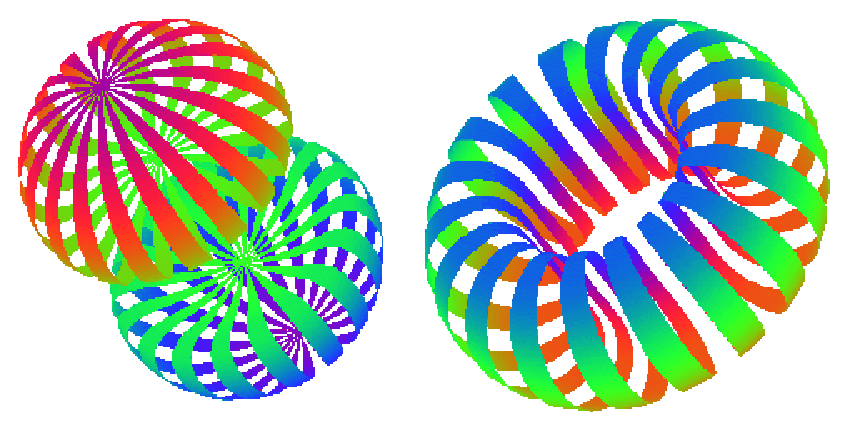
\includegraphics[width=0.5\textwidth]{figs/deuteron_states.eps}
%\caption{\label{fig:dpol-shape}
%Equidensity lines of the deuteron in its two spin projections, $M_J=\pm 1$ and $M_J=0$, respectively. Reproduced from~\cite{Carlson:1997qn,Forest:1996kp}.
%}
%\end{figure}

